
\documentclass[12pt, letterpaper]{article}
\usepackage[utf8]{inputenc}
\usepackage[margin=1in]{geometry}
\usepackage{times}
\usepackage{hyperref}
\usepackage{graphicx}
\usepackage{gensymb}
\usepackage{caption}
\usepackage{url}
\renewcommand{\abstractname}{\vspace{-\baselineskip}}

% Document
\begin{document}
\begin{center}
    \Large X-ray and Optical Solar Event Identification using Convolutional Neural Networks \\
    \vspace{.6em}
    \large Ted Grosson, Cody Meng, Preston Tracy, Jackson White
    \vspace{.3em}
    \\ Advisor: Chris Tunnell | Rice University
    \vspace{.5em}
    \normalsize
    \\ Submitted April 30, 2021
    \\
\end{center} \vspace{-2.3em}


\section*{Introduction}

Solar events\textemdash such as flares, prominences, and their associated coronal mass ejections\textemdash can lead to detrimental effects on Earth systems by disrupting electronics and communication systems, particularly in satellites with limited protection from Earth's magnetic field. Large flares can produce streams of ionized particles intense enough to harm or kill unprotected astronauts in orbiting spacecraft. Even larger flares, such as the 1859 Carrington Event famously strong enough to set fire to telegraph wires \cite{Bell2008}, pose existential threats to modern society with the potential to irreparably damage large swaths of the power grid, disable aircraft navigational and computer systems, and disrupt radio communications or military early-warning systems \cite{FlareDamage}. Given the immediacy of these threats, understanding solar events and space weather is a major scientific priority, with three U.S. organizations (the Space Weather Prediction Center, the Air Force Weather Agency, and NASA) dedicated to researching space weather systems. 

From a scientific perspective, the physical mechanisms underlying solar events are not precisely understood \cite{BOB}. Solar flares are generally classified by a peak in total solar intensity at a particular wavelength rather than by imaging of the structure of a flare. We wanted to investigate whether we could detect or classify solar events using images of the Sun rather than by simply measuring total intensity. If different types of flares carry unique observational signatures held within images of the Sun, this could hint at specific physical mechanisms underlying flares of varying types. In order to find whether these signatures of solar events exist, we use convolutional neural networks trained on thousands of multi-wavelength Extreme-Ultraviolet solar images alongside space weather reports of solar events. While the black-box nature of machine learning prevents us from obtaining a detailed understanding of the exact underlying trends, deep-learning neural nets are unparalleled at finding patterns in data. Thus, they are ideal for determining whether these patterns occur at all solar events. At this point in our project, we have been able to achieve essentially perfect validation accuracy when classifying X-ray flares despite only using images in the ultraviolet, implying that X-ray flares carry some common signature that can be used to perfectly distinguish them from other types of events. 

\subsection*{Background}

Solar flares are highly energetic events of localized ((scale citation)) increased intensity on the sun, releasing up to $10^{25}$ Joules over a time period ranging from milliseconds to over an hour \cite{BOB}. This intensity can be seen across many wavelengths, including X-ray to radio, as illustrated in Figure \ref{flare}. For comparison, Figure \ref{noflare} shows the Sun without an active event. Flares tend to be associated with groups of sunspots\textemdash localized regions of cooler material and strong magnetic fields\textemdash and are often accompanied by the ejection of charged particles, called a coronal mass ejection. The precise cause of solar flares remains uncertain, but the leading theory is that energy is suddenly released from the strong magnetic field in sunspots through a process called ``reconnection". This occurs when a magnetic field loop ``breaks" and ``reconnects" in a more stable path, releasing most of the energy stored in the loop. ((Citation))

Previous studies using AIA data tend to focus on specific details of particular events, ((such as the structure of coronal loops?)) with an emphasis on characterizing their dynamics \cite{Dai2021}\cite{Chitta2018} or their structure \cite{Aschwanden2017}. This is due to the large quantity of high quality images provided by the AIA, allowing extremely detailed studies of solar features. In contrast, our project focuses on the identification of events without intentionally isolating fine details ((of the events such as structure or intensity)). Most studies also combine AIA data with data from the Helioseismic and Magnetic Imager (HMI), which maps out the magnetic field on the solar surface \cite{Dai2021}\cite{Chitta2018}. Since solar flares are directly related to changes in the solar magnetic field, HMI data provides a simple method for searching for events. However, we would like to discover whether identification can be achieved through purely visual means, so we are not using magnetic field data from the HMI.

There have been some successful prior efforts to predict the solar flares using machine learning based on changes in the Sun’s magnetic field \cite{Raboonik2016}; however, because solar flare events are associated with changes in the Sun’s magnetic field, it has yet to be established whether they can be predicted via purely imaging techniques, although the success of this project at identifying solar X-ray flares using Extreme Ultraviolet images indicates that these images could also be used for predicting solar events.
%Should this project lead to satisfactory classification of solar events, it could provide an avenue for future predictive efforts using AIA images alongside preexisting prediction techniques.

\begin{figure}[!hb] %Pipeline figure in correct place now using !hb
	\centering
	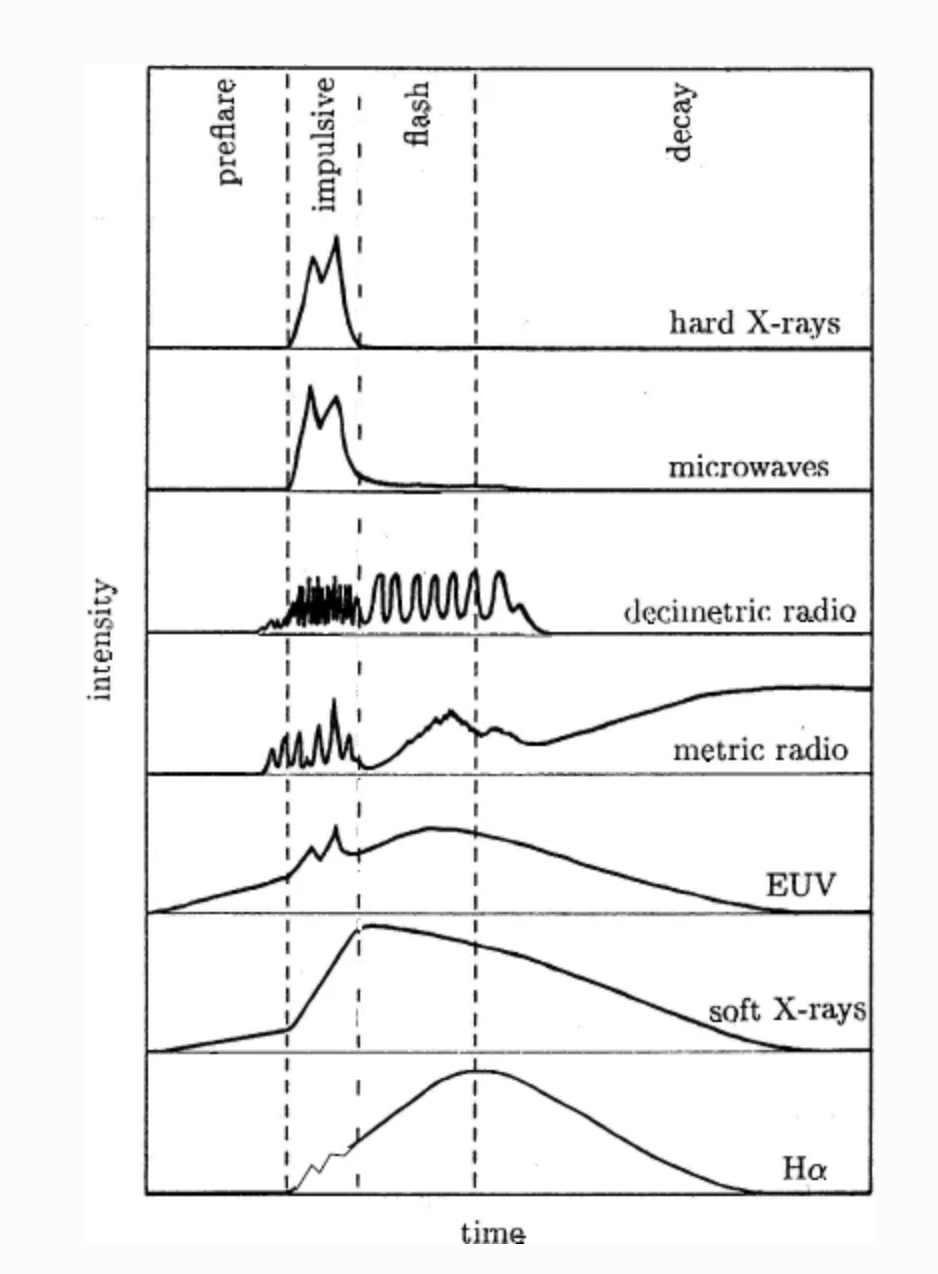
\includegraphics[width=7cm]{figures/spectra_expected.png}
    \caption{Typical Intensity vs. Time curves of X-ray flares in various wavebands \cite{Benz2008}. The waveband most relevant to our work is the EUV (Extreme Ultraviolet) spanning 1240 \AA{} to 100 \AA{}, where most of our observations lie. This suggests that our images should carry clear signatures of X-ray flares. Also worth noting in this figure is the longer buildup in EUV intensity in the preflare stage, which gives further support for using a model to predict X-ray flares. Images in from the preflare stage will show an increase in EUV intensity before the impulsive peaks in the hard X-ray wavelengths, allowing EUV images from the preflare stage to be used to forecast the more energetic impulsive stages of the flares}
    % This paragraph should probably be reworded
    \label{spectral_dist}
\end{figure}

Solar flares that peak in one wavelength are expected to have broad spectra which are visible in additional wavelengths \cite{Benz2008}. As shown in Figure \ref{spectral_dist}, X-ray flares are expected to also be visible in the EUV wavelengths that we have access to from the AIA observatory. These EUV companions should also be present at increased intensity levels both before and after the X-ray flares appear on the sun, as shown by the large temporal spread of the EUV distribution. ((This should make our goal of identifying when an X-ray flare is present a more difficult task.)) However it also indicates that it might be possible to not just identify X-ray solar flares with AIA data, but also predict their occurrence before they are visible in the X-ray wavelengths.
% State this last sentence earlier, maybe as a lead in in the introduction.

\subsection*{Objectives}

We apply machine learning image classification techniques to historical high-resolution multi-waveband solar images from the Atmospheric Imaging Assembly (AIA) in order to train a set of convolutional neural networks to identify X-ray solar events from rapid-cadence, live images of the Sun obtained by the AIA. As such, our primary objective is to produce a binary classifier capable of identifying X-ray solar events with high validation accuracy using only AIA images. 
% Took out parts relating to optical flares and future work, is there anything else that should be mentioned in this section??

%Two, we produce a binary classifier capable of identifying optical solar events with high validation accuracy using only AIA images.

%If these primary objectives are met, we may attempt to produce a tertiary neural network acting as a single multiclass classifier capable of classifying X-ray, optical, and non- events. While a natural extension of our work would be to produce a multiclass, multi-label classifier capable of categorizing all types of SWPC solar events using AIA images, the single-semester time constraint makes this infeasible. 

\subsection*{Data Science Pipeline}

% \begin{table}[h]
% 	\centering
% 	\caption*{The Pipeline}
% 	\begin{tabular}{ p{3.5cm} | p{3.5cm} | p{3.5cm} | p{3.5cm} }
% 		SWPC Reports \& AIA Images & Data Reduction & CNN Training & Validation and Classification \\ [0.5ex] 
% 		\hline
% 		Downloading & Downsizing, gzipping & Model & Validation
		
% 	\end{tabular}
% 	\vspace{0.5em}
% 	\label{Pipeline}
%     \caption{This is ugly but a quick solution.}
% \end{table}

\begin{figure}[h!]
	\centering
	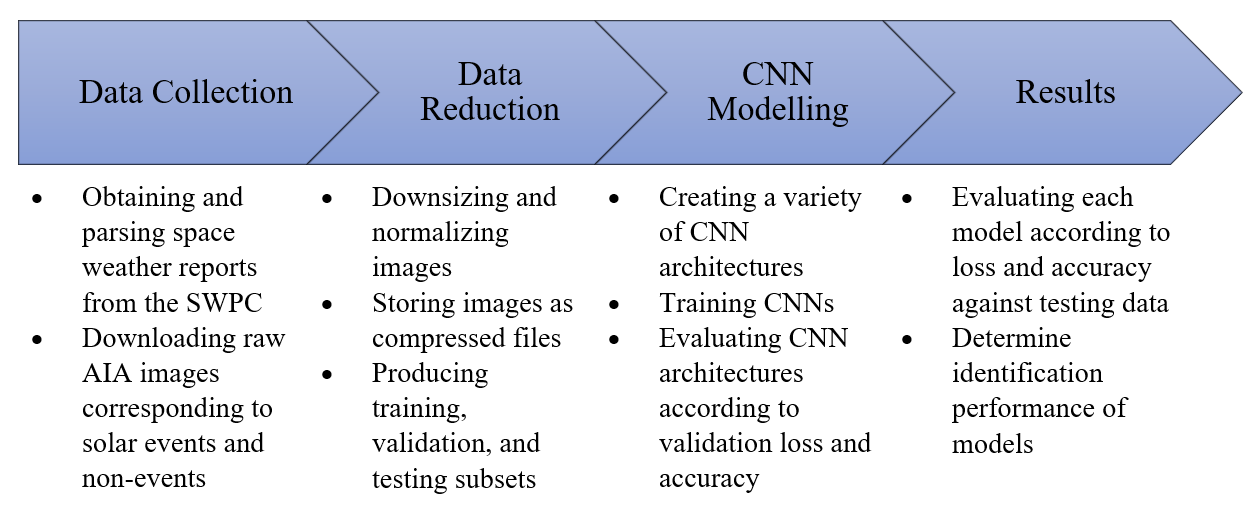
\includegraphics[width=\textwidth]{figures/pipeline.png}
	\label{Pipeline}
	\caption{Our data science pipeline, outlined. This figure outlines the different steps in our data science pipeline. The data collection step involves the processes relating to obtaining and downloading raw data from our different sources (SWPC and AIA). The data reduction step involves the "wrangling" of the raw data, or the process of turning the raw data into a form that is able to be used as inputs for our CNNs. This step involves processes such as the downsizing and normalization of the raw images and storing the images as files that can easily be loaded by the CNN. The modelling step involves the creation and training of the various CNN architectures that were tested. Finally. the results section involves the process of determining the optimal CNN structure based on accuracy and loss metrics. }
	%This figure description probably needs some rewording
\end{figure}

% Can we just have the chart be the only thing in this section or do we need some text?
% - Only the chart is necessary, see bill.com example from canvas

% Would it be better to make that vertical plot with the goals and steps?
% - do whatever, as long as it accomplishes the goal of showing each goal 
%   and step while looking nice

\section*{Data \& Data Exploration}

In this project we use two primary datasets. The first is over a decade of high-resolution, 16 megapixel images of the Sun in 10 ultraviolet and optical wavelengths taken at an approximately 12-second cadence by the Atmospheric Imaging Assembly (AIA), a solar imager located aboard the Solar Dynamics Observatory (SDO), a satellite orbiting the Earth dedicated to providing constant measurements of the Sun in order to understand solar events \cite{Pesnell2012}. The second is a database of space weather reports from the Space Weather Prediction Center (SWPC), a part of the National Weather Service (NWS) run by the National Oceanic and Atmospheric Administration (NOAA). These space weather reports catalog all detected solar events with a time, date, duration, and classification. 
% Mention how reports are made? I think that could go in the section on the reports

\begin{figure}[h!]
	\centering
	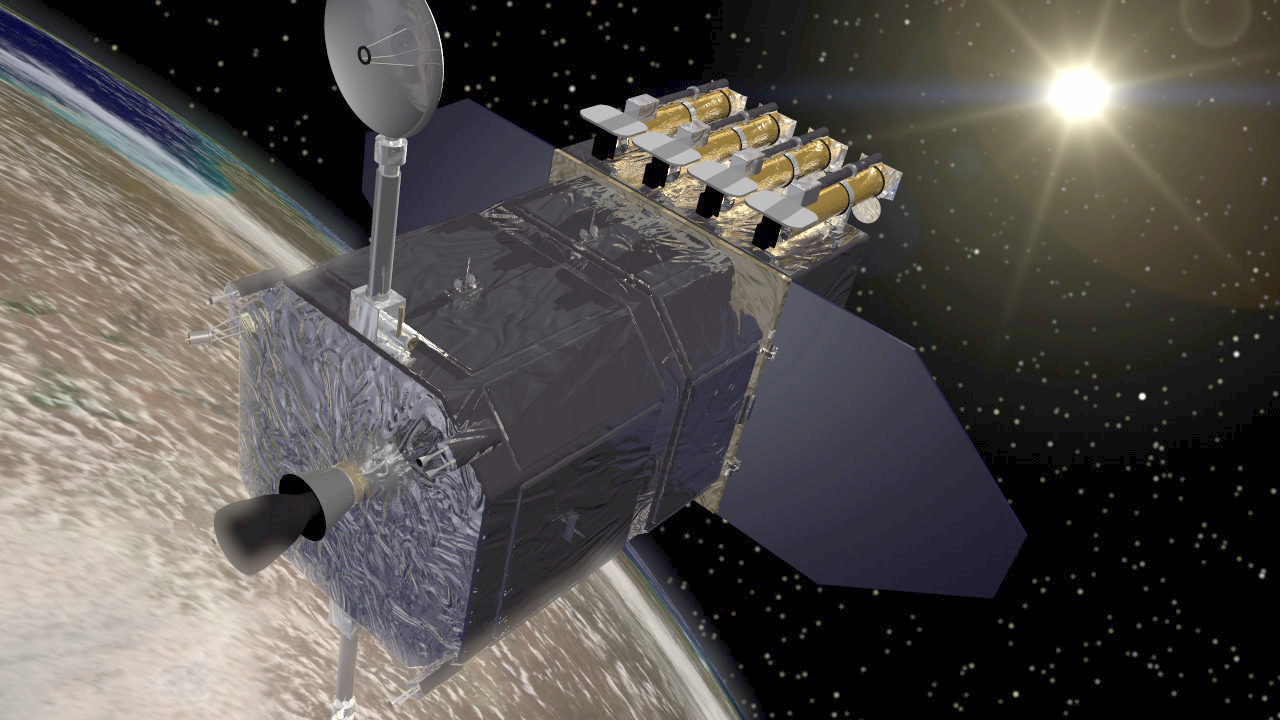
\includegraphics[width=\textwidth]{figures/sdo.jpg}
	\label{SDO}
	\caption{An artists rendering of the Solar Dynamics Observatory in orbit. The Atmospheric Imaging Assembly include the four telescopes shown facing the Sun in this image.}
	% Might need to cite the image
\end{figure}

\subsection*{AIA Observations}

% Is there an AIA reference we could include here?
The AIA takes observations at ten different wavelengths, summarized in Table \ref{AIA_wavelengths}, each probing different layers of the sun. The AIA has been observing the sun since 2010, observing at 4500~Å once per hour, at 1600 and 1700 Å once per 24 seconds (0.04166 Hz), and at the remaining wavelengths once per 12 seconds (0.0833 Hz). The images are stored as 4096$\times$4096 pixel {\scshape fits} files, a pixel array format where each pixel represents the flux captured by its corresponding pixel on the AIA camera. {\scshape fits} files also contain headers including relevant information such as exposure time and the time of the observation. These files can be queried and downloaded within Python using the {\scshape sunpy} package ((reference to sunpy??)). Using {\scshape sunpy}, we can select images based on their observation time and wavelength filter, allowing easy data access for events listed in the space weather reports.
% Would a reference to sunpy just be the documentation page?
% He says to use Hz instead of seconds for the image cadence, not sure if necessary

The different wavelengths observed by AIA were chosen to examine specific portions of the Sun’s surface or atmosphere. Each of these wavelengths are centered on a different emission line to examine the features visible at the temperature of the emission line. The EUV wavelengths observe extremely hot temperatures, and are centered on different iron ions, ranging from Fe IX (171 Å) to Fe XXIII (131 Å), and observing temperatures from $6 \times 10^4$ K (304 Å) to $2 \times 10^7$ K (193 Å) \cite{Lemen2012}. The 1700 Å and 4500 Å wavelengths show continuum images of the Sun in the UV and optical, respectively. The 1600 Å wavelength examines the transition region between the chromosphere and the corona. The 304 Å wavelength also examines the transition region, as well as the chromosphere. The 171 Å wavelength shows the “quiet” (low magnetic activity) corona and coronal loops, and the 193 Å examines a hotter region of the corona, as well as the hotter material in solar flares. The 211 Å and 335 Å wavelengths both examine the hot, magnetically active regions of the corona. Finally, the 94 Å and 131 Å wavelengths both examine flaring regions, with wavelengths centered at different temperatures \cite{Zell2015}. The temperature coverage provided by these wavelengths allows for a more complete reconstruction of thermal structure than previous missions \cite{AIA_ConceptReport}.

\begin{table}[!htb]
	\centering
	\caption*{AIA Filter Details}
	\begin{tabular}{||c| c | c | c ||}
		\hline
		Wavelength (\AA) & Emission Source & Region of Atmosphere & $\log_{10}($Temp$)$ (K)\\ [0.5ex] 
		\hline\hline
		4500 & Continuum & Photosphere & 3.7 \\
		\hline
		1700 & Continuum & Photosphere & 3.7 \\
		\hline
		1600 & C IV + Continuum & Photosphere / Transition Region & 4.7 \\
		\hline
		335 & Fe XVI & Flaring Regions & 6.8 \\
		\hline
		304 & He II & Chromosphere / Transition Region & 5.8 \\
		\hline
		211 & Fe XIV & Active-Region Corona & 6.3 \\
		\hline
		193 & Fe XII, XXIV & Corona / Hot Flare Plasma & 6.1, 7.3 \\
		\hline 
		171 & Fe IX & Corona / Transition Region & 5.0 \\
		\hline
		131 & Fe VIII, XX, XXIII & Flaring Regions & 5.6, 7.0, 7.2 \\
		\hline
		94 & Fe XVIII & Flaring Regions & 6.8 \\
		\hline
		
	\end{tabular}
	\vspace{0.5em}
	\caption{The wavelengths observed by the AIA, the primary source of emission (continuum or spectral line source) at each wavelength, the approximate layer of the Sun probed at this wavelength, and the $\log_{10}$ of the temperature, in Kelvin, of this layer. \cite{AIA_ConceptReport}}
	\label{AIA_wavelengths}
\end{table}

\subsection*{SWPC Space Weather Reports}
% Include paragraph on how the reports are made and who makes them? -CT
The second dataset, constituting thousands of space weather reports, are created once per day by the Space Weather Prediction Center (SWPC) and can contain 13 different types of space weather events, including X-ray events (XRA), optical flares (FLA), radio sweep bursts (RSP), and fixed-frequency radio bursts (RBR). These reports have been catalogued since 1997, so we have reports corresponding to all AIA data. A sample report from 2015 is depicted in Figure \ref{swr_sample}. The entire collection of reports is only 18 MB in storage size and is stored in easy-to-parse text files, so no major concerns arose when using this dataset.

Of the 13 classifications of solar events, we primarily look at 4 due to their frequency, shown in Figure \ref{swe_freq}. FLA events are flares on the solar surface peaking in the optical observed via H$\alpha$ emission, XRA events are spikes in solar X-ray flux, RBR events are narrow-band (ie. fixed frequency) radio bursts, and RSP events are radio bursts sweeping through a range of radio frequencies over the duration of the event \cite{SWPC_Glossary}. The remaining 9 categories of solar event do not appear in large enough numbers to justify their focus. In addition, these small samples may not be large enough to reliably train machine learn, especially given our emphasis on binary classification techniques.

% He said to change the title of this graphic and possibly fully expand the names on the y-axis
\begin{figure}[htb!]
    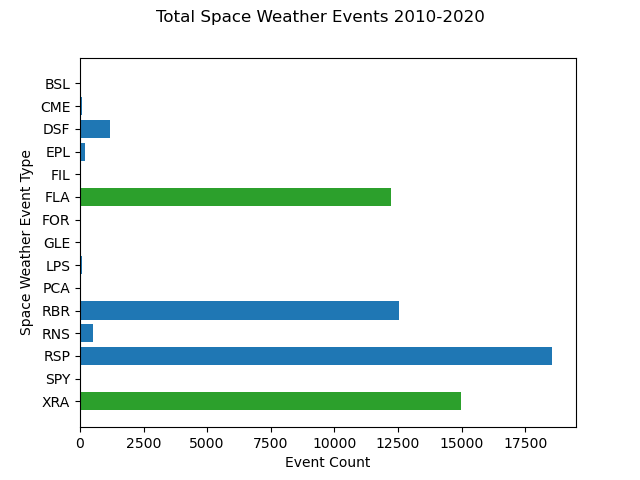
\includegraphics[width=0.9\textwidth]{figures/counts.png}
    \centering
    \caption{Total number of SWPC space weather events observed since 2010, grouped by event type, with the types used in this study highlighted in green. Of the 15 event types shown, only 4 types have large enough sample sizes to train a precise neural network|XRA, FLA, RSP, and RBR. XRA events are sharp increases in X-ray solar intensity above typical background levels due to a flare or prominence. FLA events are solar flares with intensity peaking in the optical. RSP and RBR events are bursts at radio wavelengths, with RBR (Radio Burst) events peaking at a fixed wavelength over time and RSP (Radio Sweep) events peaking at fluctuating wavelengths over time. Each of these peaks can range from factors of a few up to roughly 6 orders of magnitude above background intensity levels. At this point, we are focusing on the XRA and FLA events (highlighted in green) due to the fact that their principal wavelengths are close to the ultraviolet range of our images, unlike the radio bursts.}
    \label{swe_freq}
\end{figure}

\begin{figure}[htb!]
    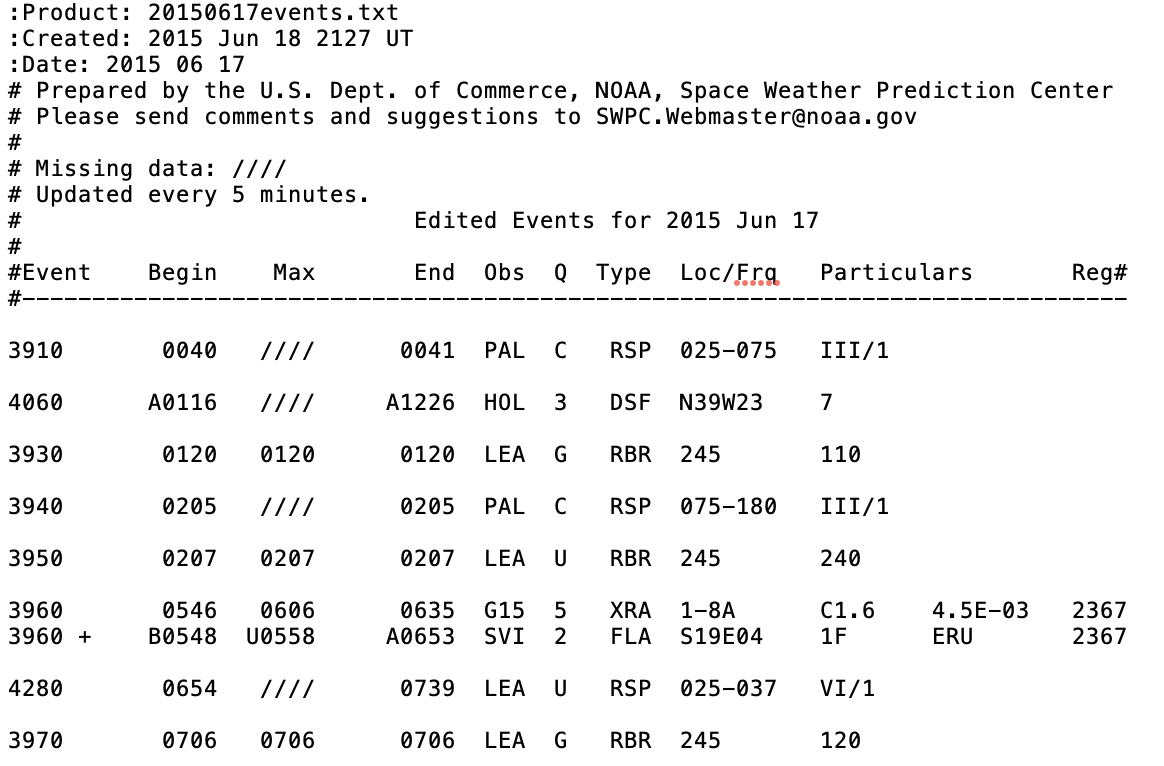
\includegraphics[width=0.9\textwidth]{figures/swr_sample.png}
    \centering
    \caption{Sample Space Weather Report text file From June 6, 2015. Along with event types and times, the reports also contain information about event locations, frequencies, and additional subclassification details. The relevant columns for this project are the "Begin" and "End" columns which denote the start and end times of events in UTC, where a time of 2:45 PM UTC would be presented as 1445 in the table. The "Obs" column denotes the observatory or satellite which observed the event in question. All XRA events are measured using the GOES satellite to determine an increase in X-Ray intensity at the Earth.}
    % This could possibly be expanded or maybe cited
    \label{swr_sample}
\end{figure}

\subsection*{Data Wrangling}

Our project was coded entirely in Python using our homemade \textit{abwoc} (Astros But WithOut Cheating) package.
%, accessible here: \hyperlink{https://github.com/PHYS477677/abwoc}{https://github.com/PHYS477677/abwoc}.

In order to generate our testing, training and validation data sets we have written python scripts which utilize the space weather reports and the sunpy python package to download and store AIA observations. These scripts download one observation per event per wavelength, for a specified event type and set of wavelengths, which are chosen at random from all the observations taken over the duration of each event which fit the specified parameters.

Each image, stored as a .fits file, is 12 MB in size, and we have approximately 60,000 observed events. This means that a full collection of images would require almost a full terabyte of storage space per wavelength. In addition, the large resolution of each image (4096$\times$4096 pixels) is unreasonably large to be used in our convolutional neural networks (CNNs) ((to be defined in the modelling section??)). To remedy both of these challenges we have written a script which iterates over our downloaded images, down samples them, and saves the underlying pixel value array as a compressed .gz file. 

The down sampling is performed as a mean pool on 8x8 arrays of pixels, reducing the resolution to 512$\times$512 pixels, and reducing the file size to about 1 MB. A resolution of 512$\times$512 pixels was chosen for two primary reasons. The first is that 512$\times$512 is the lowest resolution where we believe the relevant features on the sun, the flares that we see, retain significant detail. The difference between the two different down sampling resolutions we considered, 512$\times$512 and 1024$\times$1024, is shown in Figure \ref{resolution_1024}.


\begin{figure}[h]
	\centering
	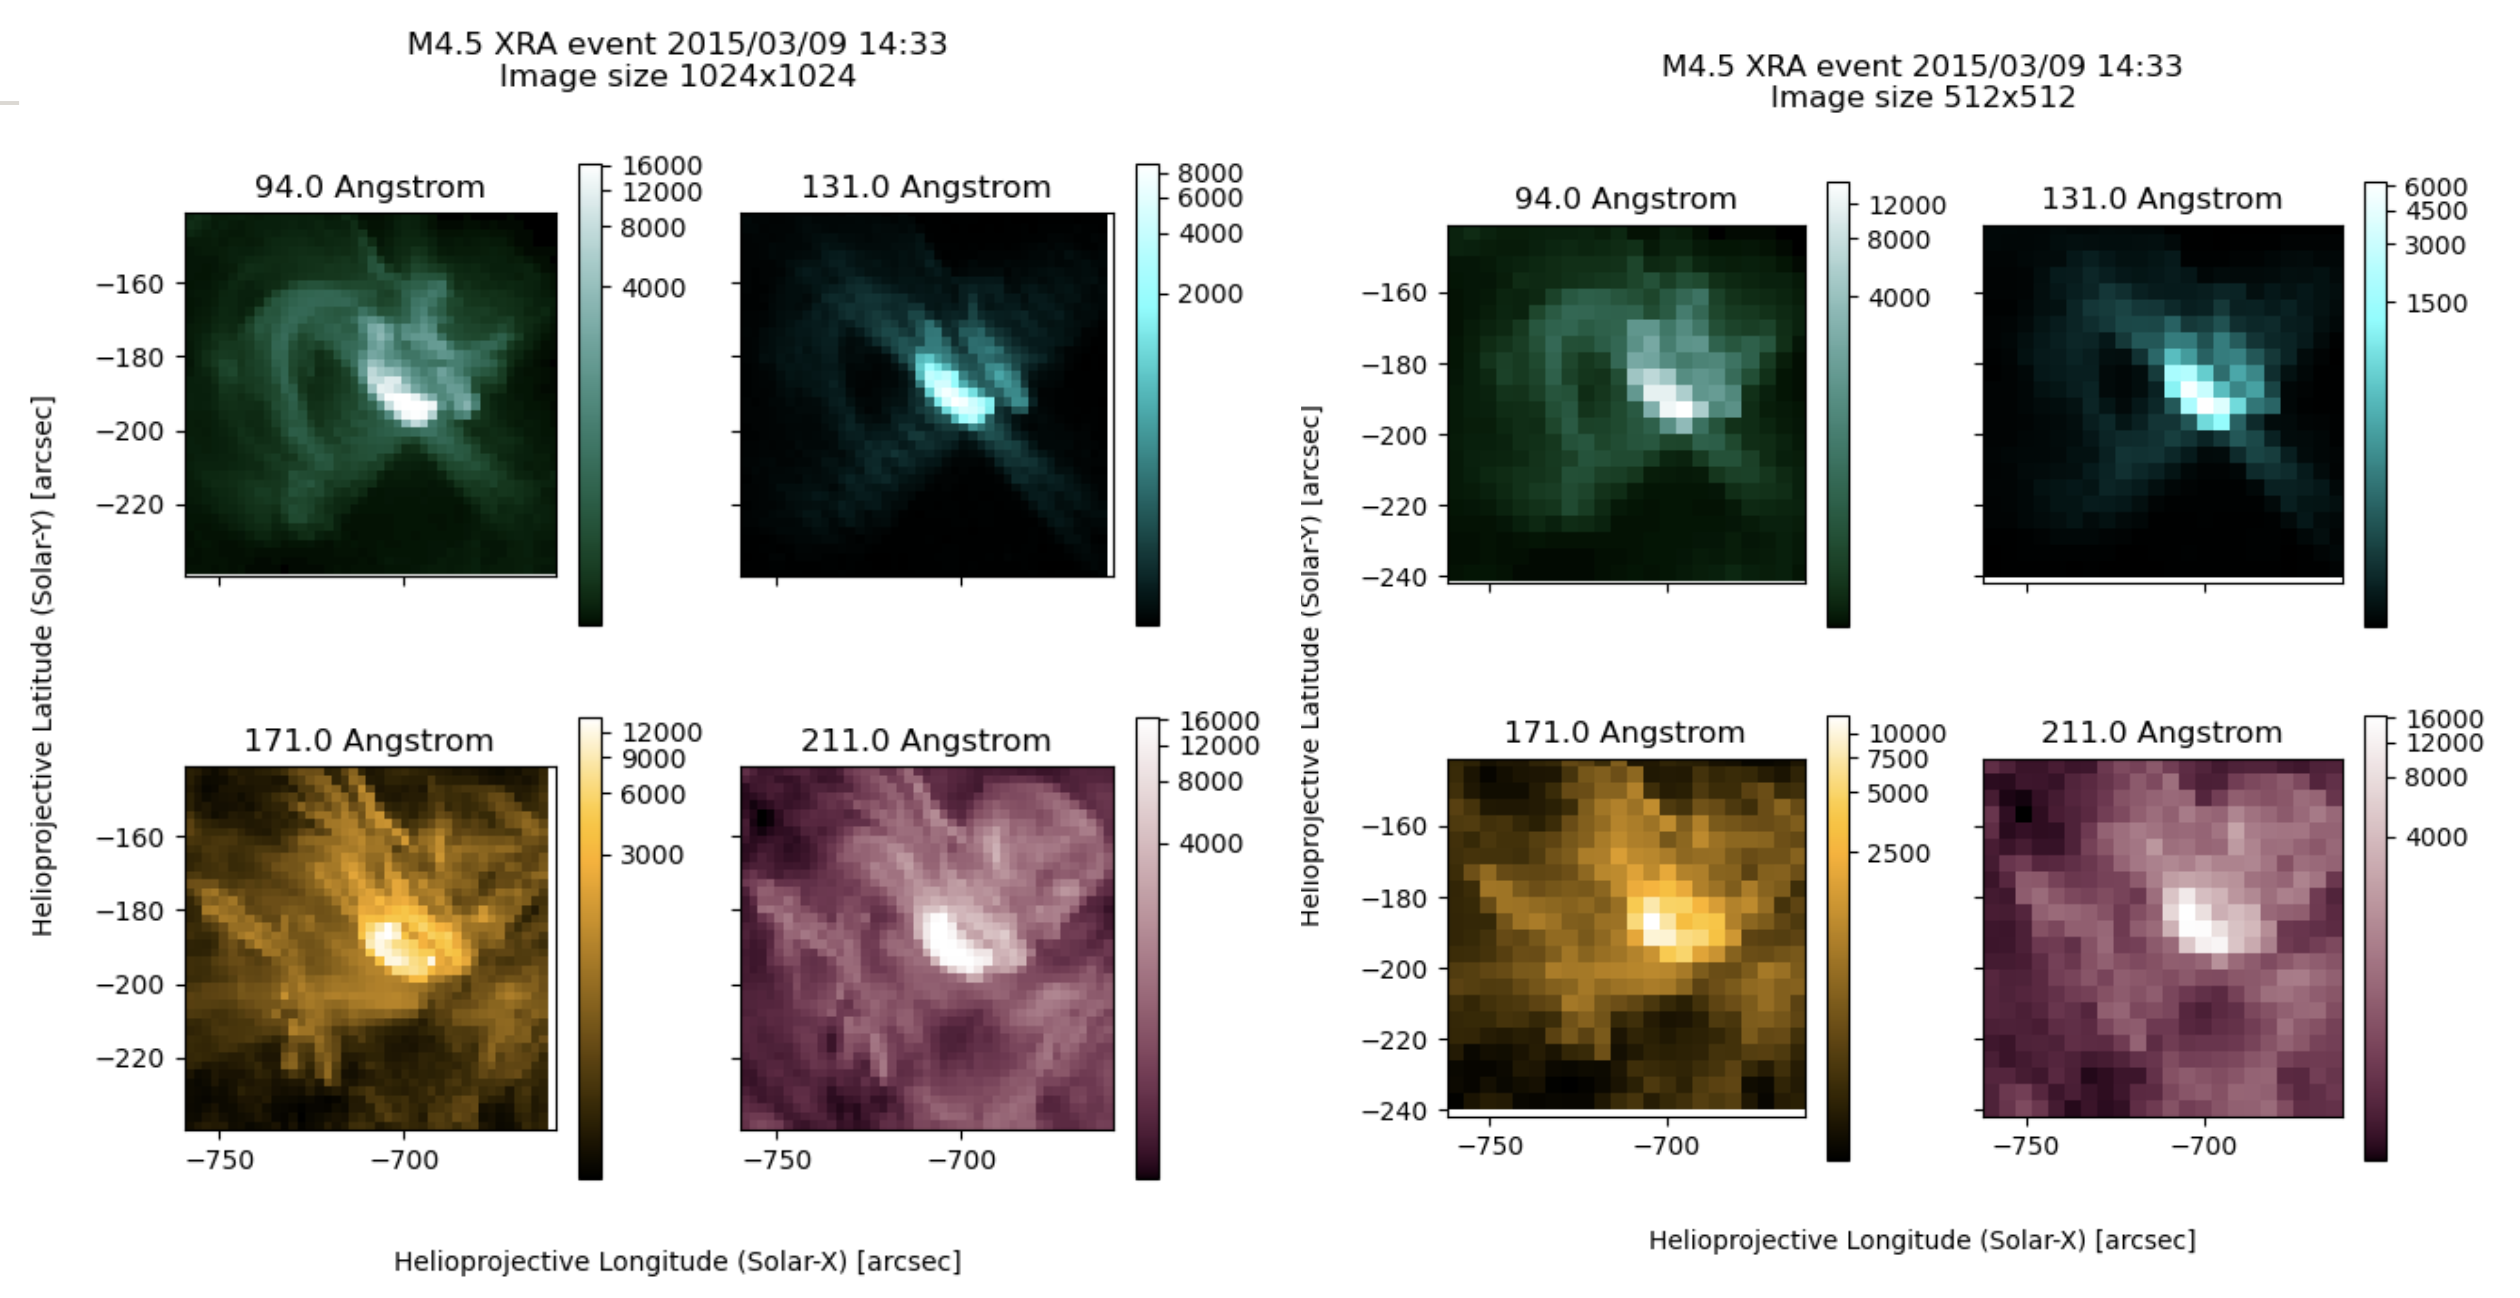
\includegraphics[width=\textwidth]{figures/resolution_demo.png}
	\caption{Resolution Comparison For A Solar Flare Feature. Left: A 1024$\times$1024 downscaled image of a solar event. Right: A 512$\times$512 downscaled image of the same solar event. Fine details are lost with downscaling, although the general structure is retained.}
	\label{resolution_1024}
\end{figure}

\subsection*{Feature Engineering}
% This is data wrangling and should possibly be moved to the data and visualization section maybe?
% Also, he complains about mentioning CNN architecture before describing CNNs, but I'm not sure what a better way to organize this would be.
CNN architecture is optimized for input values between zero and one. Although our models were able to run using unnormalized images, we chose to normalize our images for several reasons. One concern is that the model could potentially adjust its weights such that it searches only for brighter XRA events and ignores the dimmer events. Some events on the sun can be so bright that a handful of pixels are orders of magnitude brighter than the rest of the sun, make it difficult for our CNNs to learn, because bright peaks in the EUV will not necessarily originate from X-ray flares. By logarithmically normalizing our images, our CNN models are better able to make determinations and classifications based on the features seen on the surface of the sun, as shown in Figure ((#)). The loss metric is also more consistent between batches when training on normalized images. Several normalization functions were tested, and the final one chosen is shown below in Equation \ref{normfunction},
% Not sure where to put the plot showing the unnormalized CNN training

\begin{equation}
    \label{normfunction}
    n(x) = 1 - \exp\left(-\frac{x}{10\tilde{\mu}}\right)
\end{equation}
where $x$ is the initial pixel value and $\tilde{\mu}$ denotes the median pixel value of the image. Our normalization function rescales each pixel value, $x$, from [0, $\infty$) to [0, 1). The median pixel value is a robust statistic expected to be roughly consistent across images. An example of this normalization is shown in Figure \ref{norm_example}.

\begin{figure}[h]
	\centering
	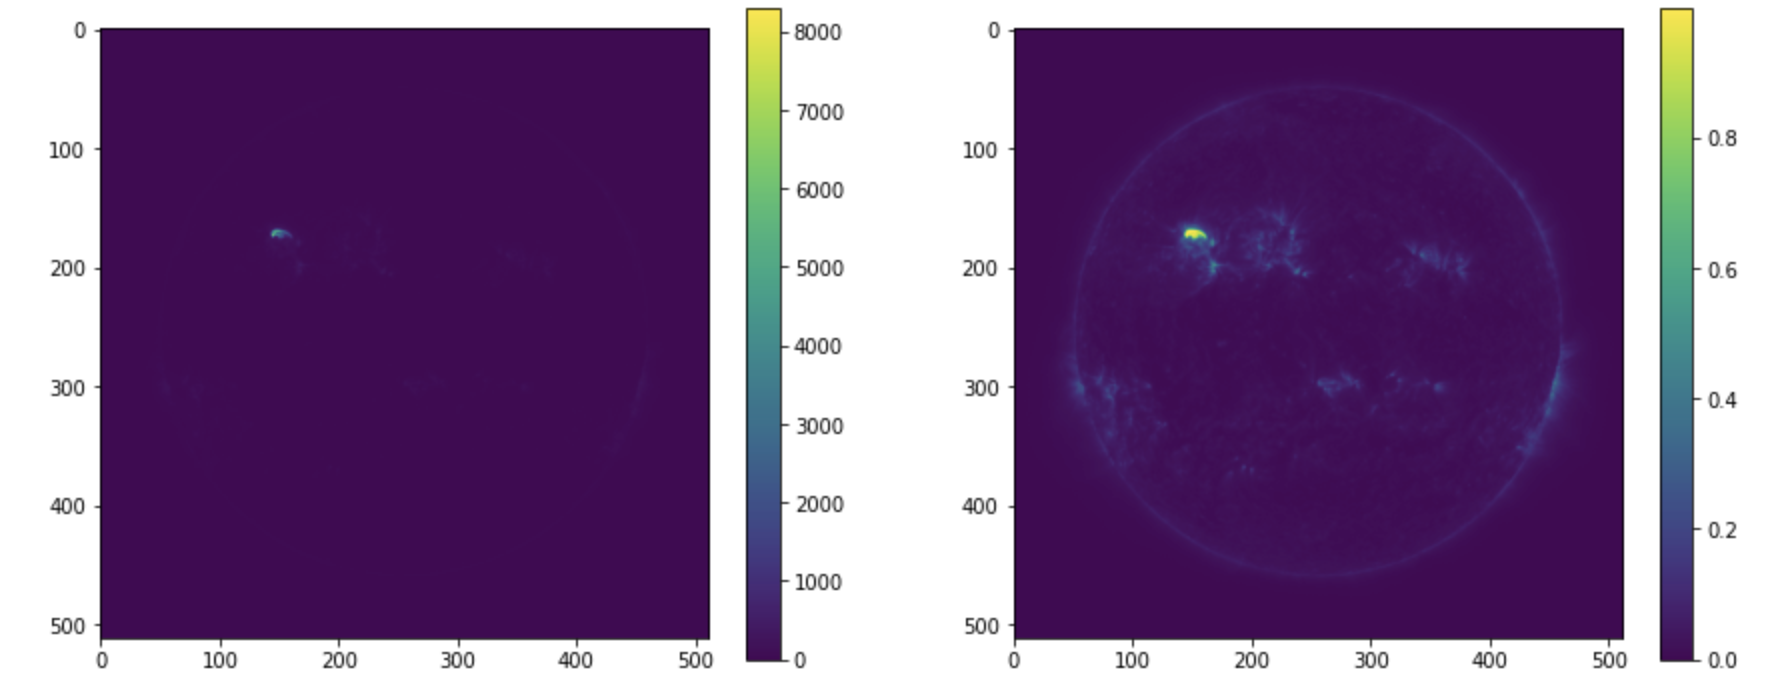
\includegraphics[width=\textwidth]{figures/normalization_comp.png}
	\caption{A typical solar image at 131Å when an X-ray flare is present. On the left is the image before normalization. On the right is the image after normalization.}
	\label{norm_example}
	% He suggests using a log axis for the colorbar of the plots, and also axis labels (or just don't include the x and y axis labels)
\end{figure}

\subsection*{Exploratory Data Analysis \& Visualization}

While exploring the space weather reports we have found 79.6\% of the reports since 2010 have at least one observed space weather event, and there are on average 15.0 events per day. There are significant frequency discrepancies between the different types of space weather events. As shown in Figure 1, the most common events are X-ray events (XRA), optical flares in H-Alpha (FLA), Sweep-Frequency Radio Bursts (RSP), and Fixed-Frequency Radio Bursts (RBR). Each of these events comprise almost a quarter of the dataset, as shown in Figure \ref{swe_freq}. Because each of these four weather types have thousands of observed events to use in our CNNs ((models?, he says not to use CNNs before defining what they are?)), and the remaining types have at most hundreds of observed events, we have decided to focus primarily on these four types of events for this project. 

Another key feature that we have identified in the data is the typical size of a visible space weather event. Most flares and prominences are on the order of about 100 pixels in each dimension, as shown in Figure \ref{event_size}. This is good because it should allow us to down sample our images considerably from their original size of 4096$\times$4096 pixels, which would be challenging to run through a CNN. 

\begin{figure}[h]
	\centering
	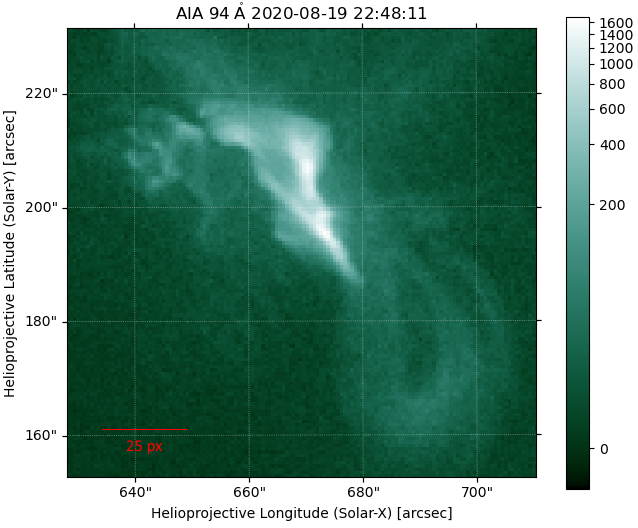
\includegraphics[]{figures/feature_scale.png}
	\caption{Typical scale for an X-ray flare. Captured in the 94 Å wavelength taken on August 8, 2020 at 10:48 UST. This image is shown in the full 4096x4096 resolution of AIA images. One arcsecond on the Sun's surface is approximately 700km, so the red scale bar in this image is about 18,000km across}
	\label{event_size}
\end{figure}


\section*{Methods \& Models}

% Should we explain more about CNNs?

\begin{figure}[h]
	\centering
	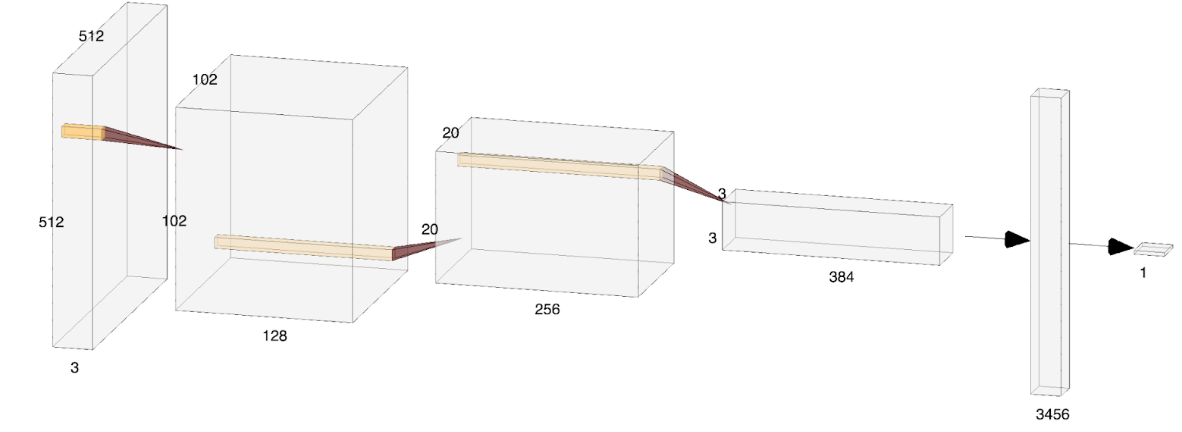
\includegraphics[]{figures/cnn_arch.png}
	\caption{The architecture of our final CNN. The initial inputs are images sized 512$\times$512 pixels in three wavelengths which are then subject to three convolution and pooling layers ((explain here or maybe in text?)), and then sent through two flatten layers? to obtain a final binary output marking a 1 if an event is present or a 0 if an event is not present.}
	% Paragraph should be reworded, and maybe the figure should be later
	\label{cnn_arch}
\end{figure}
% Probably also include a figure showing the model structure just in the Keras model.summary()

To achieve our goal of identifying solar events from AIA images, we used convolutional neural networks (CNNs) using Keras in a python environment. Because the size of the solar events in the AIA data is less than a percent of the full image, existing image identification CNN architecture could not be used to identify these solar events. Most existing image classification CNNs classify features which comprise a majority of the image, and as such are able to downsize the input images. When using a lower sized image, the CNN is able to train on images more quickly than for larger images. When attempting to train using the full 4096$\times$4096 AIA images, we found that Keras would use exorbitant amounts of memory in the training process. After downsizing the images by a factor of four to 1024$\times$1024 pixels, we found that even a simple model required over three hours to train on a set of 400 images, which is less than a tenth of our dataset. We also found that the validation accuracy obtained for these models were approximately 50\% when training on 400 images. Due to hardware limitations, primarily in memory and speed, we chose to train our models using AIA images downsized by a factor of eight to a resolution of 512$\times$512 pixels. Although there could potentially be some subtle substructure lost in the downsized images, the events still retain some visible structure at this resolution as shown in Figure 3. Additionally, our models using 512$\times$512 pixel images were able to train on a dataset containing four thousand images over four epochs in the same time a model would require to train on four hundred images using the 1024$\times$1024 pixel images.

% The normalization discussion should go in feature engineering

There were several different model architectures tested when creating our CNN. We tested both simple and “deep learning” neural networks. Conceptually, a single layer neural network would be effective if there are a limited number of ways that an event can appear in our data. In contrast, a multi-layer or deep learning model would build up the structure of features across several layers, which would potentially gain more insight into the structure of various events. An additional parameter considered when creating model structures was the number of wavelengths used. Different wavelengths are able to analyze different layers in the atmosphere of the Sun, and therefore different structure in solar events. Through the use of images in multiple wavelengths, a model could potentially better identify events by incorporating features from all wavelengths used. If the multi-wavelength model did not perform significantly better than a single wavelength model, then the increased RAM usage and training time required to train a multi-wavelength model would make the single wavelength model more optimal to use. 

Our main metric used to measure the effectiveness of a certain model was the validation accuracy, with other secondary factors taken into consideration such as the speed or memory usage of a model. When training our models, we also aimed to reduce overfitting, which occurs when the validation loss is significantly higher than the training loss. Overfitting is a sign that the model is fitting too closely to the training dataset, and not identifying the structure of the desired features.

\section*{Results}

For both single wavelength images, as well as multi-wavelength images, we find that the ``deep-learning" CNN models, preform significantly better than simple single or two-convolution layer models. The deep-learning CNN models, which contain at least three layers of convolutions and max-pooling, take longer to over fit and reach higher validation accuracy values. This is demonstrated in Figure \ref{CNN_171_2}, which uses a two convolution layer model trained on 171 angstroms and Figure \ref{CNN_171_3} which uses three convolution layers.

XRA events do appear to carry some signature visible to a neural network that distinguish them from other types of events or non-events likely held within the multiple wavelength information. 65-75\% validation accuracy is possible with single-wavelength models, but this is improved when applying multiple wavelengths. 

One possible reason for the high multi-wavelength accuracy is that, because XRA events emit light predominantly in the X-ray, XRA events will have a higher intensity at bluer wavelengths than redder wavelengths. In contrast, the Sun's peak wavelength is in the optical, so in the ultraviolet wavelength range, bluer wavelengths will have a weaker intensity than redder wavelengths. This suggests that X-ray events would have a different intensity relationship with wavelength than the background surface of the Sun, which the neural network could be using to identify these events. If this is the case, then optical flares may be more difficult to identify, as this inverted relationship does not hold for an event peaking in the optical.

When we began using three wavelength images we found a sudden jump in the success of our CNN. Our three wavelength CNN found an almost 7 order of magnitude downward jump in loss value, and reached 100\% validation. An example of this is attached in the appendix as figure \ref{flare_bug}. However, these results now appear to have been caused by an incorrect creation of our training data set. While this is disappointing, it does align more with our initial expectations that creating an essentially perfect identifier would be very difficult to achieve, especially given that EUV prominences can both precede X-Ray bursts, and last longer than X-Ray bursts, as shown in figure \ref{spectral_dist}. 
% Including old plots in case we can't recreate the old ones before thursday:
% Don't know what the best way to display these would be

%\begin{figure}[ht]
%	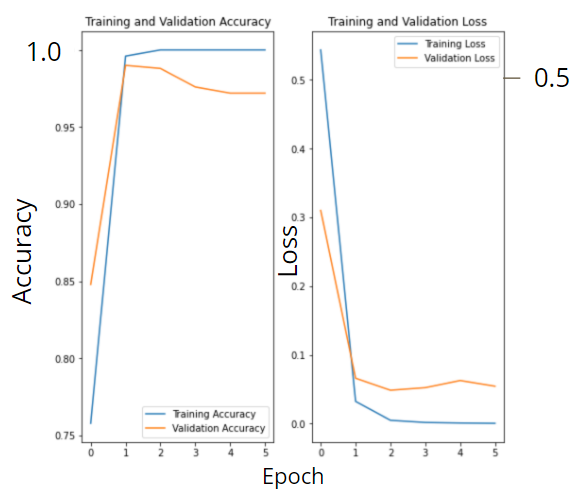
\includegraphics[width=\textwidth]{figures/three_onelayer.png}
%	\centering
%	\caption{Model with one convolution layer trained using images in %the 131 Å, 171 Å, and 211 Å wavelengths}
%	\label{CNN_3_1}
%\end{figure}

\section*{Conclusion \& Future Work}

From our results, we have established that solar X-ray events can be reliably identified from images of the Sun in the ultraviolet wavebands using convolutional neural networks. 

Currently, we plan to extend this binary classification CNN modeling to optical flare (FLA) events. The main bottleneck when attempting to add different types of events is the time required to download and downsample additional images. This process takes about three weeks (assuming a dataset of three thousand or so images) for each additional event classification. The time required during the training and modeling steps are negligible in comparison to data acquisition and wrangling. 

Once we obtain a large enough optical flare dataset, we also plan to produce a multiclass classification scheme capable of identifying both optical and X-ray events in a single neural network. This would likely be our final product for the semester.

The natural conclusion of this work would be a multiclass, multi-label classifier for all 13 SWPC categories of solar events, ideally using all 10 AIA wavelengths. A Multi-label classifier would be able to handle overlapping solar events, which likely take up a non-negligible portion of the data set. Alternative methods avoiding the use of convolutional neural nets, such as spectral index analysis or applying simple intensity thresholds may also be able to produce good results. Attempting to isolate which features our models are using to classify these events may also prove fruitful. 

\bibliographystyle{unsrt}
\bibliography{bibfile}
\pagebreak
\section*{Appendix}

\begin{figure}[h]
	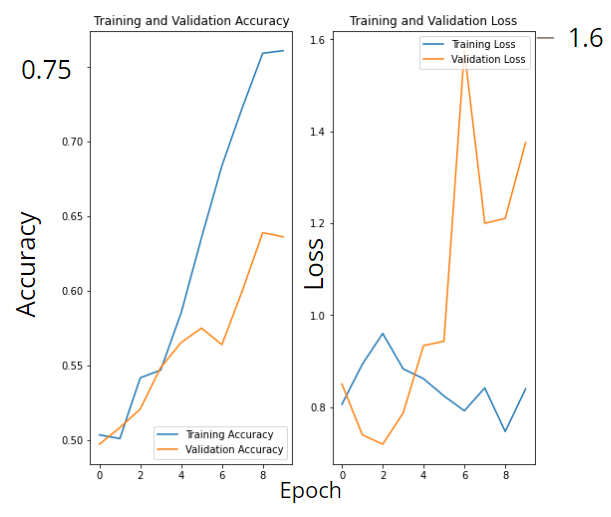
\includegraphics[width=\textwidth]{figures/171_twolayer.png}
	\centering
	\caption{Model with two convolution layers trained using images in the 171 Å wavelength}
	\label{CNN_171_2}
\end{figure}

\begin{figure}[h]
	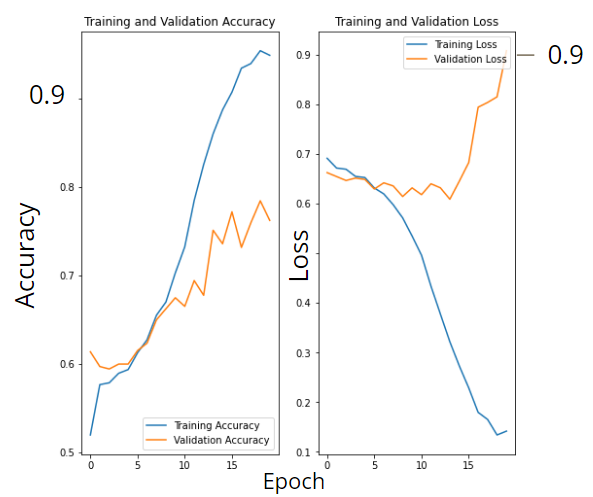
\includegraphics[width=\textwidth]{figures/171_threelayer.png}
	\centering
	\caption{Model with three convolution layers trained using images in the 171 Å wavelength}
	\label{CNN_171_3}
\end{figure}


\begin{figure}[h]
	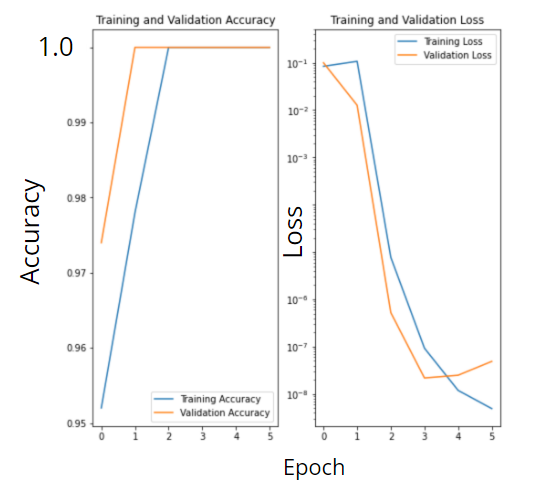
\includegraphics[width=\textwidth]{figures/three_threelayer.png}
	\centering
	\caption{Model with three convolution layers trained using images in the 131 Å, 171 Å, and 211 Å wavelengths, which now appears to have been caused due to a bug in our code}
	\label{flare_bug}
\end{figure}

\begin{figure}[ht]
	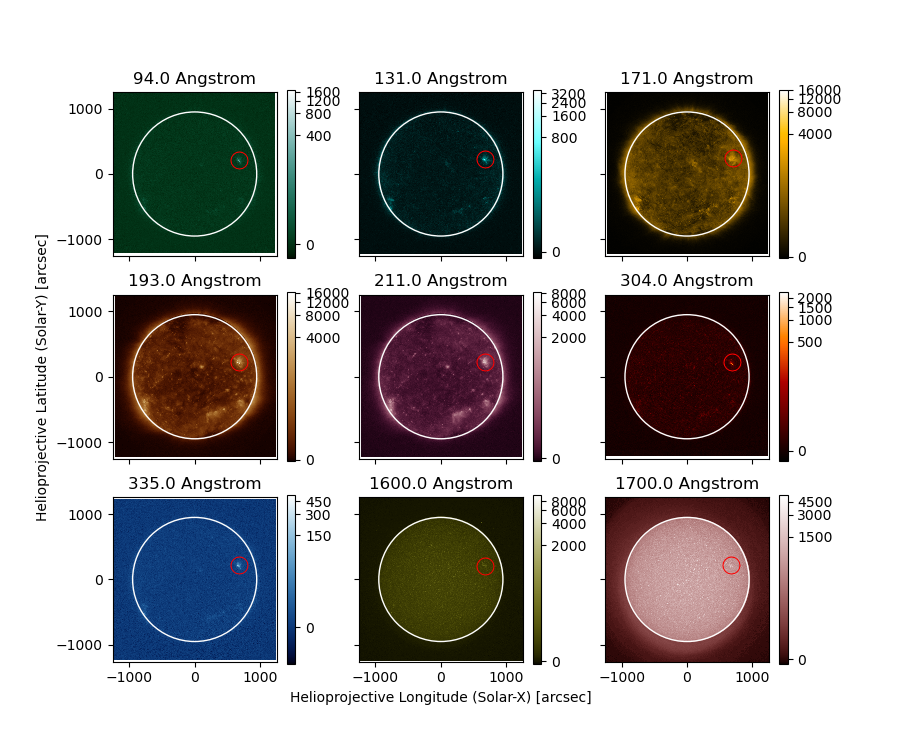
\includegraphics[width=\textwidth]{figures/0819_flare_labeled.png}
	\centering
	\caption{A small X-ray flare which occurred August 19, 2020 in each AIA wavelength apart from 4500~\AA{}. The flare, circled in red on each image, shows up in all wavelengths to varying degrees.}
	\label{flare}
\end{figure}

\begin{figure}[ht]
	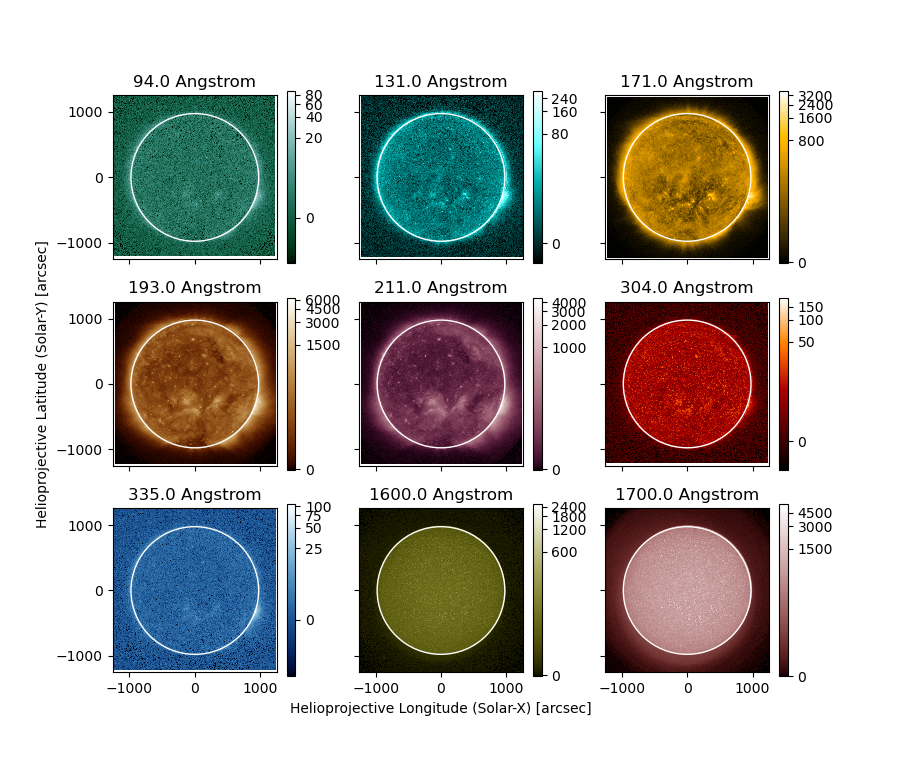
\includegraphics[width=\textwidth]{figures/noflare.png}
	\centering
	\caption{The Sun in each wavelength without an active flare. Note the much smaller colorbar scales than in the image above.}
	\label{noflare}
\end{figure}

\begin{table}[h!]
	\begin{center}
		\begin{tabular}{||c | c ||} 
			\hline
			Acronym & Full Name \\ [0.5ex] 
			\hline\hline
			BSL & Bright Surge on Limb \\
			\hline
			CME & Coronal Mass Ejection \\ 
			\hline
			DSF & Filament Disappearance \\ 
			\hline
			EPL & Eruptive Prominence on Limb\\
			\hline
			FIL & Filament\\
			\hline
			FLA & Optical Flare in H-Alpha\\
			\hline
			FOR & Forbush Decrease (CR Decrease) \\
			\hline
			GLE & Ground-Level Event (CR Increase) \\
			\hline
			LPS & Loop Prominence System\\
			\hline
			PCA & Polar Cap Absorption\\
			\hline
			RBR & Fixed-Frequency Radio Burst\\
			\hline
			RNS & Radio Noise Storm\\
			\hline
			RSP & Sweep-Frequency Radio Burst\\
			\hline
			SPY & Spray\\
			\hline
			XRA & X-ray Event \\
			\hline
		\end{tabular}
		\caption{List of Event Types tracked in space weather reports}
		\label{space_weather_events}
	\end{center}
\end{table}

\end{document}


